\chapter{Sort}


\section{Introduction}
List of general algorithms:
\begin{enumerate}
\item Selection sort: invariant
\begin{enumerate}
\item Elements to the left of $i$ (including $i$) are fixed and in ascending order (fixed and sorted).
\item No element to the right of $i$ is smaller than any entry to the left of $i$ ($A[i]  \leq\min(A[i+1:n])$.
\end{enumerate}
\item Insertion sort: invariant
\begin{enumerate}
\item Elements to the left of $i$ (including $i$) are in ascending order (sorted).
\item Elements to the right of $i$ have not yet been seen.
\end{enumerate}
\item Shell sort: h-sort using insertion sort.
\item Quick sort: invariant
\begin{enumerate}
\item $|A_p|..\leq..|..unseen..|..\geq..|$ maintain the 3 subarrays.
\end{enumerate}
\item Heap sort: compared to quick sort it is guaranteed $O(N \lg N)$, compared to merge sort it is $O(1)$ extra space. 
\end{enumerate}

\section{Algorithms}
\subsection{Quick Sort}
\subsubsection{Normal pivoting}
The key part of quick sort is pivoting:
\begin{python}
def pivot(self, A, i, j):
    """
    pivoting algorithm:
    p | closed set | open set |
    | closed set p | open set |
    """
    p = i
    closed = p
    for ptr in xrange(i, j):
        if A[ptr] < A[p]:
            closed += 1
            A[ptr], A[closed] = A[closed], A[ptr]

    A[closed], A[p] = A[p], A[closed]
    return closed
\end{python}

Notice that this implementation goes $O(N^2)$ for arrays with all duplicates.

\textbf{Problem with duplicate keys}: it is important to stop scan at duplicate
keys (counter-intuitive); otherwise quick sort will goes $O(N^2)$ for the
array with all duplicate items, because the algorithm will put all items
equal to the $A[p]$ on \textbf{a single side}. 

Example: quadratic time to sort random arrays of 0s and 1s.

\subsubsection{Stop-at-equal pivoting}
Alternative pivoting implementation with optimization for duplicated keys:
\begin{python}
def pivot_optimized(self, A, lo, hi):
    """
    Fix the pivot as the 1st element
    Scan from left to right and right to left simultaneously
    Avoid the case that the algo goes O(N^2) with duplicated keys
    """
    p = lo
    i = lo
    j = hi
    while True:
        while True:
            i += 1
            if i >= hi or A[i] >= A[lo]:
                break
        while True:
            j -= 1
            if j < lo or A[j] <= A[lo]:
                break

        if i >= j:
            break

        A[i], A[j] = A[j], A[i]

    A[lo], A[j] = A[j], A[lo]
    return j

\end{python}
\subsubsection{3-way pivoting}
3-way pivoting: pivot the array into 3 subarrays: 

$|..\leq..|..=..|..unseen..|..\geq..|$ 
\begin{python}
def pivot_3way(self, A, lo, hi):
    lt = lo-1  # pointing to end of array LT
    gt = hi  # pointing to the end of array GT (reversed)

    v = A[lo]
    i = lo  # scanning pointer
    while i < gt:
        if A[i] < v:
            lt += 1
            A[lt], A[i] = A[i], A[lt]
            i += 1
        elif A[i] > v:
            gt -= 1
            A[gt], A[i] = A[i], A[gt]
        else:
            i += 1

    return lt+1, gt
\end{python}

\subsection{Stability}
Definition: a stable sort preserves the \textbf{relative order of items with equal keys} (scenario: sorted by time then sorted by location). 

Algorithms:
\begin{enumerate}
\item Stable
\begin{enumerate}
\item Merge sort
\item Insertion sort
\end{enumerate} 
\item Unstable
\begin{enumerate}
\item Selection sort
\item Shell sort
\item Quick sort
\item Heap sort
\end{enumerate}
\end{enumerate}
\textbf{Long-distance swap} operation is the key to find the unstable case during sorting. 
\begin{figure}[hbtp]
\centering
\subfloat{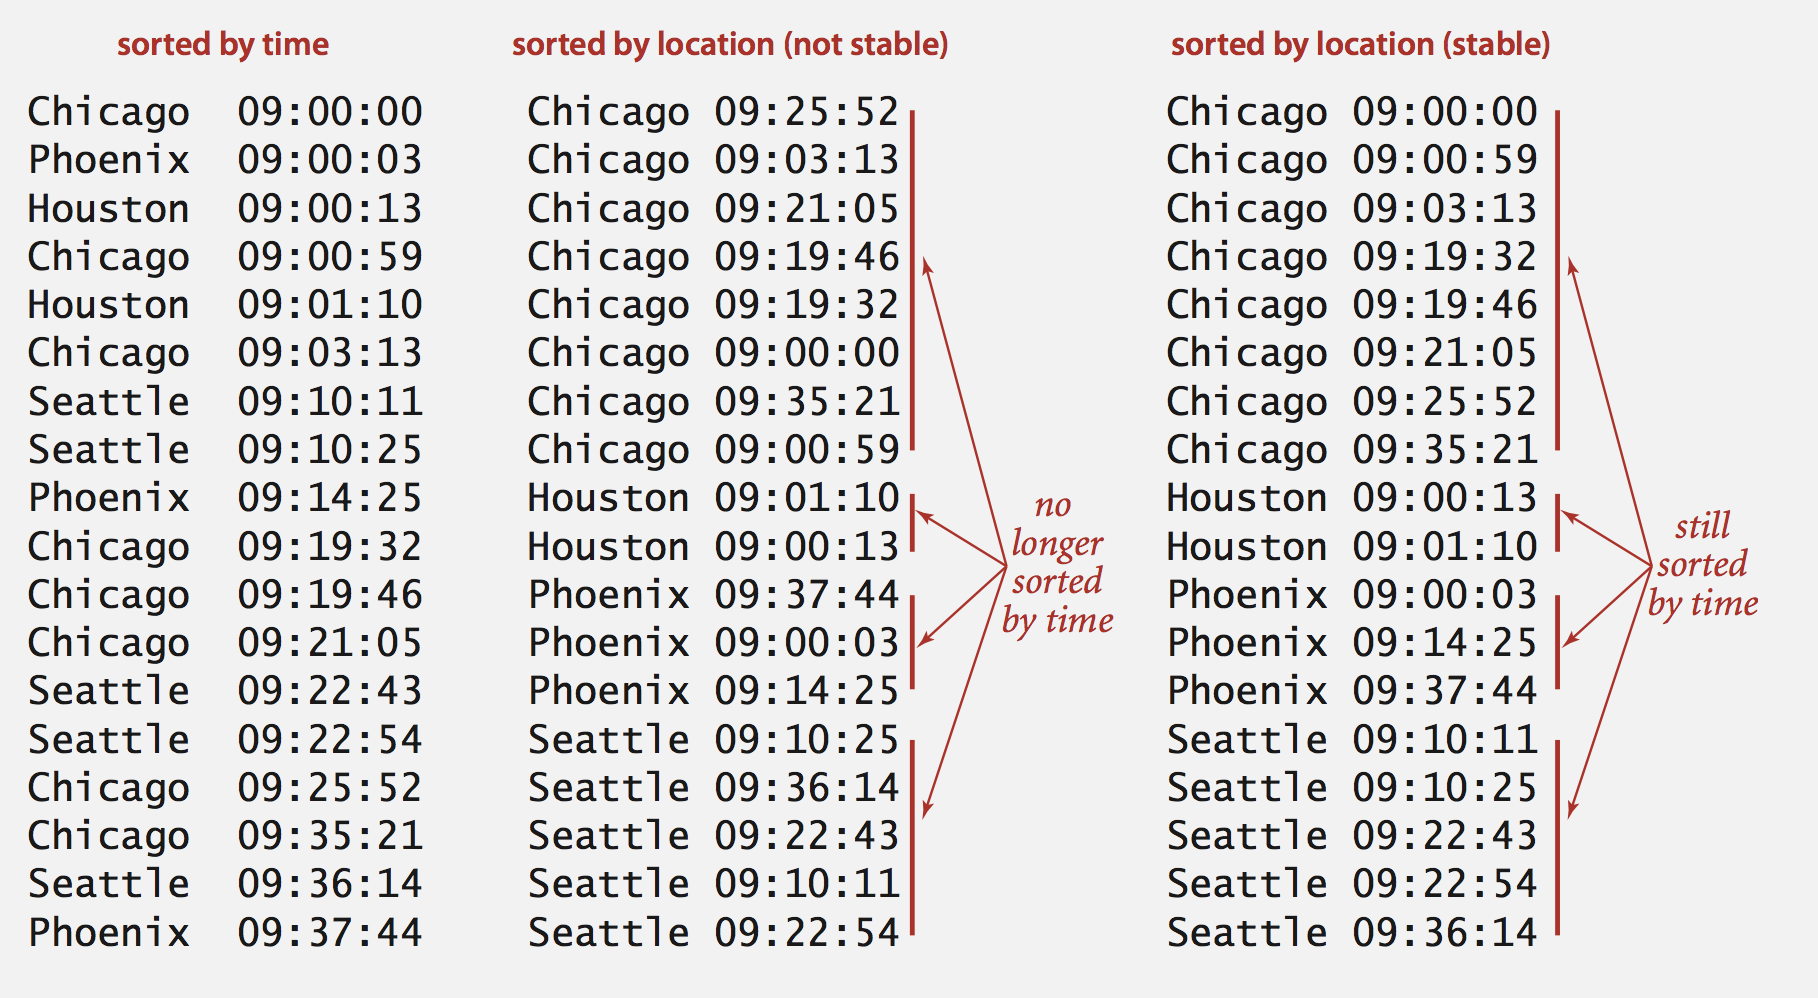
\includegraphics[scale=.60]{stable_sort}}
\caption{Stale sort vs. unstable sort}
\label{fig:trie} 
\end{figure}

\subsection{Applications}
\begin{enumerate}
\item Sort
\item Partial quick sort (selection), k-th largest elements 
\item Binary search
\item Find duplicates 
\item Graham scan
\item Data compression
\end{enumerate}

\subsection{Considerations}
\begin{enumerate}
\item Stable?
\item Distinct keys?
\item Need guaranteed performance?
\item Linked list or arrays?
\item Caching system? (reference to neighboring cells in the array? 
\item Usually randomly ordered array?
(or partially sorted?)\item Parallel?
\item Deterministic?
\item Multiple key types?
\end{enumerate}

$O(N\lg N)$ is the lower bound of comparison-based sorting; but for other
contexts, we may not need $O(N \lg N)$:
\begin{enumerate}
\item Partially-ordered arrays: insertion sort to achieve $O(N)$. \textbf{Number of inversions}: 1 inversion $=$ 1 pair of keys that are out
of order.
\item Duplicate keys
\item Digital properties of keys: radix sort to achieve $O(N)$.
\end{enumerate}

\subsection{Summary}
\begin{figure}[hbtp]
\centering
\subfloat{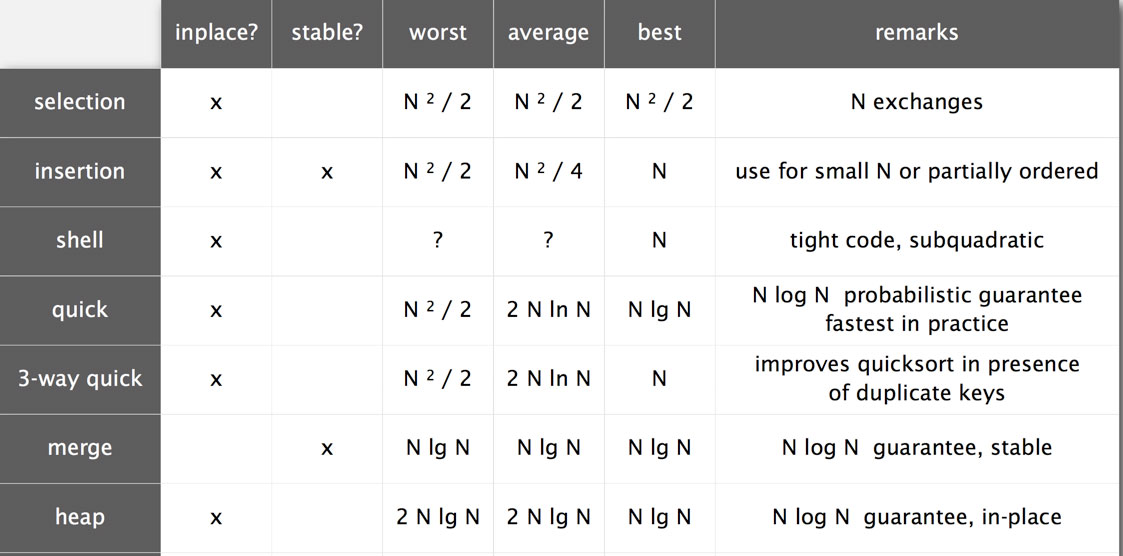
\includegraphics[scale=0.80]{sort_summary}}
\caption{Sort summary}
\label{fig:trie} 
\end{figure}


\section{Inversion}
If $a_i > a_j$ but $i<j$, then this is considered as 1 Inversion. 

\subsection{MergeSort \& Inversion Pair}
MergeSort to calculate the \#reverse-ordered paris. The only difference from a normal
merge sort is that - when pushing the 2nd half of the array to the place, you calculate
the inversion generated by the element $A_2[i_2]$ compared to $A_1[i_1:]$.

\begin{python}
def merge(A1, A2, A):
  i1 = i2 =0
  ret = 0
  for i in xrange(len(A)):
    if i1 == len(A1):
      A[i] = A2[i2]
      i2 += 1
    elif i2 == len(A2):
      A[i] = A1[i1]
      i1 += 1
    else:
      # use array diagram to illustrate
      if A1[i1] > A2[i2]:  # push the A2 to A
        A[i] = A2[i2]
        i2 += 1
        # number of reverse-ordered pairs
        ret += len(A1) - i1
      else:
        A[i] = A1[i1]
        i1 += 1

  return ret

def merge_sort(a):
  n = len(a)
  if n == 1:
    return 0

  a1 = a[:n/2]
  a2 = a[n/2:]

  ret1 = merge_sort(a1)
  ret2 = merge_sort(a2)
  # merge not merge_sort
  ret = ret1+ret2+merge(a1, a2, a)  
  return ret
\end{python}

\subsection{Binary Index Tree \& Inversion Count}
Given $A$, calculate each element's inversion number. 

Construct a BIT (\ref{BIT}) with length $max(A)+1$. Let BIT maintains the index of values. Scan the element from left to right (or right to left depends on the definition of inversion number), and set the index equal val to 1. Use the prefix sum to get the inversion number.

$get(end)-get(a)$ get the count of number that appears before $a$ (i.e. already in the BIT) and also larger than $a$. 

Possible to extend to handle duplicate number. 
\\
Core clues:
\begin{enumerate}
\item BIT maintains \textbf{index of values} to count the number of at each value.
\item $get(end)-get(a)$ to get the inversion count of $a$.
\end{enumerate}
\begin{python}
def inversion(self, A):
    bit = BIT(max(A)+1)
    ret = []
    for a in A:
        bit.set(a, 1)  # += 1 if possible duplicate 
        inversion = bit.get(max(A)+1) - bit.get(a)
        ret.append(inversion)

    return ret
\end{python}

\subsection{Reconstruct Array from Inversion Count}\label{inversionReconstruct}
Given a \textit{sorted} numbers with their associated inversion count (\# larger numbers before this element). $A[i].val$ is the value of the number, $A[i].inv$ is the inversion number. Reconstruct the original array $R$ that consists of each $A[i].val$.

Brute force can be done in $O(n^2)$. Put the $A[i].val$ into $R$ at an index/slot s.t. the \# \textit{empty} slots before it equals to $A[i].inv$.

\rih{BST}. Possible to use BST to maintain the empty slot indexes in the original array. Each node's rank indicates the count of empty indexes in its left subtree. But need to maintain the deletion.  

\rih{Segment Tree}. Use a segment tree to maintain the size of empty slots. Each node has a $start$ and a $end$ s.t slot indexes $\in [start, end)$. Go down to find the target slot, go up to decrement the size of empty slots. 

Code:
\begin{python}
class Node(object):
  def __init__(self, start, end, cnt):
    self.start = start
    self.end = end
    self.cnt = cnt

    self.left = None
    self.right = None

  def __repr__(self):
    return repr("[%d,%d)" % (self.start, self.end))


class SegmentTree(object):
  """empty space"""
  def __init__(self):
    self.root = None

  def build(self, start, end):
    """a node can have right ONLY if has left"""
    if start >= end:
      return

    root = Node(start, end, end-start)
    root.left = self.build(start, (end+start)/2)
    if root.left: 
      root.right = self.build((start+end)/2, end)
    return root

  def find_delete(self, root, val):
    """
    :return: index
    """
    root.cnt -= 1
    if not root.left:
      return root.start
    elif root.left.cnt >= val:
      return self.find_delete(root.left, val)
    else:
      return self.find_delete(root.right, 
                              val-root.left.cnt)


class Solution(object):
  def reconstruct(self, A):
    st = SegmentTree()
    n = len(A)
    st.root = st.build(0, n)
    A = sorted(A, key=lambda x: x[0])
    ret = [0]*n
    for a in A:
      idx = st.find_delete(st.root, a[1]+1)
      ret[idx] = a[0]

    return ret

if __name__ == "__main__":
  A = [(5, 0), (2, 1), (3, 1), (4, 1,), (1, 4)]
  assert Solution().reconstruct(A) == [5, 2, 3, 4, 1]
\end{python}
